\documentclass[11pt]{article}
\usepackage[utf8]{inputenc}
\usepackage{amsmath, amsthm, amssymb}
\usepackage[letterpaper, margin=1in]{geometry}
\usepackage{microtype}
\usepackage{enumitem}
\usepackage{biblatex}
\usepackage{mathtools}
\usepackage{amssymb}
\usepackage{float}
\usepackage{commath}
\usepackage{color, soul}
\usepackage{wrapfig}
\usepackage{xfrac}
\usepackage{hyperref}

\addbibresource{main.bib}

\newtheorem{theorem}{Theorem}[section]
\newtheorem{corollary}{Corollary}[theorem]
\newtheorem{lemma}[theorem]{Lemma}
\newtheorem{alg}[theorem]{Algorithm}
\newtheorem{claim}[theorem]{Claim}

\theoremstyle{definition}
\newtheorem{definition}{Definition}[section]

\theoremstyle{definition}
\newtheorem{subroutine}{Subroutine}

% Commonly used symbols
\newcommand{\R}{\mathbb{R}}
\newcommand{\fu}{f^{\mu}}
\newcommand{\nfi}{\nabla f_i}
\newcommand{\nfiu}{\nabla \fu_i}
\newcommand{\biu}{b_{i}^{\mu}}
\newcommand{\gij}{\gamma_{ij}}
\newcommand{\geu}{\gamma_e^{\mu}}
\newcommand{\giij}{\gamma_{ij}^{\mu}}
\newcommand{\vnott}{V \setminus t}
\newcommand{\din}{\delta^{\text{in}}}
\newcommand{\dout}{\delta^{\text{out}}}
\newcommand{\vsrc}{V^{s}}
\newcommand{\vsink}{V^{t}}
\newcommand{\vz}{V^{0}}
\newcommand{\fp}{(f,\mu)}
\newcommand{\fiju}{f_{ij}^{\mu}}

\newcommand{\xands}{X \cap S}
\newcommand{\xnots}{X \setminus S}

\DeclareMathOperator{\Ex}{Ex}
\DeclareMathOperator{\Def}{Def}

\newcommand{\rewrite}[1]{\textcolor{red}{#1}}
\newcommand{\todo}[1]{\hl{TODO: #1}}

\newcommand{\lpeq}[1] {
\begin{equation*}
\begin{aligned}
#1
\end{aligned}
\end{equation*}
}
\newcommand{\lpone}[3] {
& \underset{}{\text{#1}}
&& #2 \\
& \text{s.t.}
&& #3 
}
\newcommand{\lptwo}[4] {
\lpone{#1}{#2}{#3}\\
&&& #4
}
\newcommand{\lpthree}[5] {
\lptwo{#1}{#2}{#3}{#4}\\
&&& #5
}

\title{Strongly Polynomial Algorithms for Generalized Flow Maximization}
\author{Francis Cangialosi, Katie Lewis, David Palmer}
\date{}

\begin{document}
\maketitle
\section{Introduction}
	\subsection{Problem Definition}
	As in the traditional flow problem, given a
	graph $G = (V,E)$, the generalized maximum flow problem aims to maximize the
	total flow delivered to the sink node $t \in V$. Unlike the original flow
	problem however, each edge contains a gain factor $\gamma_e > 0$, which scales
	the flow passing through that edge. Intuitively, this scaling can be thought
	of in terms of real world examples such as exchange rates between currencies
	or physical transformations due to energy dissipation. The generalized maximum
	flow problem lacks several nice properties that are present in the traditional
	maximum flow problem, which makes it more challenging to solve. For example,
	the generalized problem is usually thought to be \rewrite{non-integral} and,
	due to the gain factors, the total supply is not necessarily equal to the total
	demand. Additionally, the maximum flow-minimum cut theorem no longer applies
	since the flow along a path is not equal at every edge along that path.
    
	Until recently, the best known algorithms were all weakly polynomial. In
	2013, \cite{Vegh2013} developed the first strongly polynomial algorithm
	(i.e. one that depends only on the number of nodes and edges in the graph,
	and is independent of the size of their values). In 2017, \cite{Olver2017}
	built on this work and developed an algorithm that is faster by a factor of
	almost $O(n^2)$, resulting in a running time that is as fast as the best
	weakly polynomial algorithms even for small parameter values. These
	algorithms take advantage of the structural similarities between the
	generalized maximum flow problem and the minimum cost flow problem by
	adapting techniques from well-known combinatorial min cost flow algorithms.
    
	\subsection{Structure and Contributions of the Paper}
	In this paper, we aim to
	familiarize the reader with the recent algorithmic developments for the
	generalized flow maximization problem and provide intuition for the techniques
	used to achieve a strongly polynomial result. In Section 2, we more formally
	define the problem as a linear program and give an overview of the notation
	used in the rest of the paper. In Section 3, we develop the key techniques
	shared by both algorithms used to achieve a strongly polynomial bound for this
	problem. In Section 4, we describe Végh's original $O(n^3m^2)$ strongly
	polynomial algorithm developed in 2014 and present a more intuitive and
	detailed analysis than the original paper. In Section 5, we describe Olver and
	Végh's faster $O((m + n\log n)mn\log(n^2 / m))$ algorithm and highlight key
	aspects of the analysis that led way to the improved running time efficiency.
	Finally, in Section 6, we conclude with open questions and present a few ideas
	for future work.
	\todo{Update when we're done.}
    
\section{Preliminaries}

	\subsection{Network Notation}
	%An instance of the generalized flow problem is specified as	
	Let $G=(V,E)$ be a directed graph with $n=\abs{V}$ and $m=\abs{E}$,
	$t \in V$ be a sink node and $\gamma \in \R_{>0}^E$ be the vector of flow gains
	across the edges. Although we have typically seen flow constraints defined in terms of
	edge capacities, recent work on the generalized problem defines flow
	constraints using node demands $b \in \R^{V \setminus t}$ instead (and leave
	edge capacities unbounded). Thus, an instance of the generalized flow problem
	is specified as $(G, t, \gamma, b)$.
	We adopt this formulation in our paper for
	convenience of analysis. As shown in~\cite{Vegh2013}, any problem defined with
	node demands can be easily transformed to an equivalent problem with
	capacities. 

	Although there is no explicit specification of a source node, the concept of
	node demands generalizes the concept of having multiple sources and multiple
	sinks: nodes with negative demand $-b$ act as sources because they can create
	up to $b$ units of flow, and nodes with positive demand $b$ act as sinks 
	because they consume at least $b$ units of flow. Thus, (excluding $t$), we denote the subset of
	vertices with negative demand as $\vsrc$, the subset of vertices with positive
	demand as $\vsink$, and the remaining nodes with zero demand as $\vz$.

	For a subset of the vertices $S \subseteq V$, we define $\din(S)$ and
	$\dout(S)$ to be the set of incoming and outgoing edges, respectively,
	and let $d_i = |\din(\{i\}) \cup \dout(\{i\})|$ be the total degree of a
	node $i \in V$.

	Then we can define the net flow at a node $i$ as the amount of flow that
	reaches a node (scaled by the gain factor on the incoming edges) minus the
	amount of flow that leaves the node: 
	$$ \nfi \coloneqq \sum_{e \in \din(i)} \gamma_e f_e - \sum_{e \in \dout(i)} f_e.$$

	The residual graph $G_f = (V,E_f)$ is defined as in the traditional problem,
	except the reverse residual edges $(j,i) \in E_f$ have inverted gain 
	$\gamma_{ji} = 1 / \gamma_{ij}$ and negated flow $f_{ji} =
	-\gamma_{ij}f_{ij}$. If the cumulative gain of a cycle $C$ ($\prod_{e \in C} \gamma_e$)
	in $G_f$ is greater than 1, we call $C$ a ``flow-generating cycle.'' 
	This captures the idea of arbitrage: sending a unit of flow around the cycle
	generates a net surplus.





	\subsection{Linear Program Formulation}
	\label{sec:lp}

	We formulate the generalized flow maximization problem with demands as in the 2017
	paper~\cite{Olver2017}:
	\vspace{-0.35cm}
%		\begin{align*}
%		\text{max} \quad
%		\nabla f_t& \\
%		\text{s.t.} \quad \tag{P}
%		\nabla f_i &\geq b_i \quad \forall i \in V \setminus t \\
%		f &\geq 0
%		\end{align*}        
%
%		\noindent The dual of (P) is shown below on the left. If we set
%		\rewrite{$\mu = \mu$}, we arrive at the formulation on the right,
%		as given in~\cite{Olver2017}:
%

    \begin{align*}\tag{P}
    \text{max} \quad
    \nabla f_t& \\
    \text{s.t.} \quad
    \nabla f_i &\geq b_i \quad \forall i \in V \setminus t \\
    f &\geq 0
    \end{align*}

	The dual linear program, given on the left below, has a variable $\eta_i$ for
	every vertex $i$. 
	Making the change of variables $\eta_i = - \mu_t / \mu_i$ yields the
	dual optimization problem on the right.

	\begin{tabular}{rcll}
		\hspace*{-1.05cm}
	\resizebox{0.37\textwidth}{!}{
		\fbox{
	\begin{minipage}{0.35\textwidth}
	\begin{alignat*}{3}
    \text{min} &\quad &\sum_{i \in V \setminus t} b_i \eta_i \\
    \text{s.t.}
    &   &\gij \eta_j - \eta_i &\geq 0 \quad &&\forall\; (i, j) \in E[V \setminus t] \\
    &   &\gamma_{ti} \eta_i &= -1 \quad     &&\forall\; (i, t) \in E \\
    &   &\eta_i &= -\gamma_{it} \quad       &&\forall\; (t, i) \in E \\
    &   &\eta_i &\leq 0 \quad               &&\forall\; i \in V \setminus t
    \end{alignat*}
	\end{minipage}
}
} & 
	$\xrightarrow{\hspace*{0.25cm}\eta_i = - \mu_t / \mu_i\hspace*{0.25cm}}$
	&
	\resizebox{0.37\textwidth}{!}{
		\fbox{
	\begin{minipage}{0.4\textwidth}
    \begin{alignat*}{3}
    \text{max} &\quad &\mu_t &\sum_{j \in V \setminus t} \frac{b_j}{\mu_j}  \\
    \text{s.t.}
    &   &\gij \mu_i &\leq \mu_j \quad &&\forall\; (i, j) \in E \\
    &   &\mu_i &\in \R_{>0} \cup \infty \quad &&\forall\; i \in V \setminus t \\
    &   &\mu_t &\in \R_{>0}
    \end{alignat*}
	\end{minipage}
}
} & \hspace*{0.4cm}(D)
\end{tabular}

        
	A dual solution $\mu$ is known as a \emph{labeling}, and we can speak of feasible and
	optimal labelings. As long as the sink is reachable from every vertex, $\mu$ will be finite.
	Complementary slackness requires that for an optimal flow $f^*$ and labeling $\mu^*$,
	any edge $(i, j)$ with flow on it ($f^*_{ij} > 0$) has $\gamma_{ij}\mu^*_i = \mu^*_j$.
	This suggests a particular interpretation of the dual variables. Imagine that
	the vertices represent currencies and the gains represent exchange rates between those currencies.
	A maximum generalized flow is the currency trading strategy that maximizes the value in currency
	$t$ at the end. We can interpret a label $\mu_i$ as the value of one dollar in currency $i$.
	The dual constraint $\gamma_{ij} \mu_i \leq \mu_j$ means that under the labeling $\mu$,
	it is not possible to create value by converting currencies.
	The complementary slackness condition means that the currency trading strategy
	only makes use of the best exchange rates, those that exactly preserve value.
	
	Given a dual solution, we can transform the gains and demands to obtain a new
	problem instance. Given a feasible flow, we can also transform the flow values
	so that they will be feasible for the transformed instance:
	\[ f_{ij}^\mu \coloneqq \frac{f_{ij}}{\mu_i} \quad
	\nabla f_i^\mu \coloneqq \frac{\nabla f_i }{\mu_i} \quad
	\gamma_{ij}^\mu \coloneqq \gamma_{ij} \frac{\mu_i}{\mu_j} \quad
	b_i^\mu \coloneqq \frac{b_i}{\mu_i} \]
	The transformed problem is equivalent to the original problem.
	
	An edge $e$ is known as \textbf{tight} with respect to $\mu$ if $\gamma_e^\mu =1$.
	For an optimal pair $(f, \mu)$, complementary slackness is exactly the condition that
	flow only flows along tight edges. We denote the set of all tight edges under
	$\mu$, $\{\geu = 1\ \forall\ e  \in E\}$, as $\tau(\mu)$. \todo{check that
	this is used consistently everywhere}
	
	Given flow values and labels, the total excess and deficit of the flow with respect
	to the labels is defined as follows:
	\begin{align*}
	\Ex(f,\mu)  &\coloneqq \sum_{i \in V \setminus t} \max \{ \nfiu - \biu, 0 \} \\
	\Def(f,\mu) &\coloneqq \sum_{i \in V \setminus t} \max \{ \biu - \nfiu, 0 \}
	\end{align*}
  
\section{Motivating Ideas and Techniques}
	\subsection{Solving Dual}
    	%* Talk about idea of solving dual 
      %  	* Key insight about this algorithm is that they maintain $f^{\mu}$ (without any extra work apparently) to be integral
      %      * Allows normal flow algorithms 
      %      * Is maintaining solution that is "close enough to feasible primal" with complementary slackness unique to this algorithm?
      %      * Draw parallels between min cost flow and generalized max flow (give more clear and intuitive explanation than the Truemper paper)
            
	The algorithm \todo{explain which algorithm(s)} solves the primal generalized flow problem by first solving the dual problem.
    A solution to the dual problem specifies, by complementary slackness, the edges on which an optimal
    primal solution may send flow. Moreover, applying the dual labels regularizes the problem, reducing
    it to an ordinary circulation problem. Starting from dual labels $\mu$, $f^{\mu}$ must satisfy
    \[ \sum_{j \in \din(i)} \giij \fu_{ij} - \sum_{j \in \dout(i)} \fu_{ji}
     = \nabla f^{\mu} \geq b^{\mu}, \]
    but $\giij = 1$ whenever $f_{ij} \neq 0$. Therefore the dual solution reduces the primal problem
    to an ordinary maximum flow problem with demand constraint.
    
    In fact, modulo an ordinary maximum flow computation, the dual problem reduces to computing
    the set of tight edges. Since regular maximum
    flow has already been solved in strongly polynomial time, it suffices to find a strongly polynomial
    algorithm to compute a set of tight edges consistent with a dual optimal solution. This problem
    is inherently combinatorial, suggesting that it can be solved in strongly polynomial time.
    
    \subsection{Contracting edges}
    To organize the search for tight edges, the algorithm inductively reduces the graph.
    Suppose an edge $(i, j)$ is known to be tight for any dual-optimal solution $\mu$. This
    imposes a constraint $\giij = 1$ for all such $\mu$, or, i.e., $\gij \mu_i = \mu_j$.
    Imposing a constraint of this form reduces the dimension of the solution
    space by one and is equivalent to removing one variable from optimization. Indeed,
    suppose we solve the equivalent problem instance $(\biu, \giij)$. Then the new constraint
    becomes $\mu_i' = \mu_j'$. In order to avoid working with extra constraints, we might
    as well remove one of the variables entirely by collapsing the edge $(i, j)$, leaving a single
    vertex $j$ with a single dual variable $\mu_j$. It remains to set the demand $b_j$ so
    that the problem remains equivalent. Rewritten in terms of the variables in
    the modified problem, the relevant terms of the dual objective are
    \[ \mu_t' \left(\frac{b_i^\mu}{\mu_i'} + \frac{b_j^\mu}{\mu_j'}\right)
     = \mu_t' \left(\frac{b_i^\mu + b_j^\mu}{\mu_j'}\right). \]
	So the operation of collapsing $i$ into $j$ along $(i, j)$ and summing their demands
	preserves the objective and constraints.
	
	The algorithm adds one additional simplification: if the contraction leads to parallel edges,
	only the one with the highest gain is maintained. This is motivated by the primal problem: in
	the absence of edge capacity constraints, there is no reason to send flow along an edge of
	lower gain when one of higher gain is available. Thus, culling parallel edges preserves the
	essential features of the problem.
	
	\subsection{Certificates}
	Complementary slackness tells us that if there is a primal optimal flow $f$ with
	$f_e > 0$, then $e$ is tight with respect to \emph{every} dual optimal solution---that
	is, $e$ is contractible. So a primal optimal flow provides a certificate for contractibility.
	It would seem this is of no use to us, as computing a primal optimal flow is the entire
	problem we are trying to solve. However, an optimal flow is a vastly superfluous certificate.
	Note that we only need to know that \emph{some}
	primal optimal flow is supported on one particular edge $e$.
	
	Suppose we had any flow $g$, and we could bound the difference between $g$ and an optimal
	flow $f^*$. Then if $g$ had a sufficiently large value on some edge $e$, we would know that
	$f^*_e \neq 0$.
	
	In fact, the algorithm goes one step further. Instead of maintaining a feasible flow
	fitting the dual solution $\mu$, it maintains a ``pseudoflow'' along with a guarantee
	that there is a feasible flow also fitting $\mu$. In order for this to work, $\mu$
	must be such that a feasible flow fitting it exists, even if that flow is never
	computed. If this condition holds, $\mu$ is called \emph{safe}. An equivalent
	formulation of safety, which is easier to reason about, is as follows. To simplify
	the exposition, we define 
	\begin{definition}
		Given dual labels $\mu$, an \textbf{inward-loose cut} is a set $S \subseteq V$ such that
		$\din(S) \cap E^\mu = \varnothing$. An \textbf{outward-loose cut}
		is such that $\dout(S) \cap E^\mu = \varnothing$. A \textbf{bi-loose cut}
		is both inward- and outward-loose.
	\end{definition}
	If $f$ is a flow fitting $\mu$, then there is no flow into inward-loose cuts.
	If $f$ is feasible, then it follows that the total demand inside an inward-loose
	cut is negative. It turns out that this is a sufficient condition for the existence
	of a feasible fitting flow.
	\begin{lemma}[Certificate for Safety] \label{lem.safety}
	$\mu$ is safe if and only if for any inward-loose cut $S$,
	\[ \sum_{i \in S} \biu \leq 0. \]
	\end{lemma}
	This is Lemma 2.3 in \cite{Olver2017}, where it is described as a corollary of Hoffman's Circulation
	Theorem, Theorem 11.2 in \cite{Schrijver2002}. We provide a proof for completeness:
	\begin{proof}
		Suppose the cut condition holds. Let $f$ be a function on tight edges minimizing
		the total deficit $\Def(f, \mu) = \sum_i \min\{0, \biu - \nfiu\}$. Let
		$T^+$, $T^-$ be the sets of vertices with excess and deficit, respectively:
		\begin{align*}
			T^+ &= \{i \in V \mid \nfiu > \biu \} \\
			T^- &= \{i \in V \mid \nfiu < \biu \}.
		\end{align*}
		Consider the residual graph of $f$ in the tight graph. If there were a path
		connecting $T^+$ to $T^-$, then we could augment along the path
		to reduce the total deficit. Therefore, there is no such path. Consider the
		set $T$ of nodes from which $T^-$ is reachable along tight edges (including reverse edges).
		The absence of a residual path from $T^+$ to $T^-$
        implies that $T \cap T^+ = \varnothing$, whence
		\[ \sum_{i \in T} \nfiu - \biu = \sum_{i \in T^-} \nfiu - \biu < 0. \]
		By definition, $T$ is inward-loose. Therefore, the total flow into $T$ is zero.
        Moreover, the total flow out of $T$ is zero, for otherwise there would be
        residual tight edges into $T$. So
		\[ 0 = \sum_{e \in \din(T)} f_e - \sum_{e \in \dout(T)} f_e
		     = \sum_{i \in T} \nfiu < \sum_{i \in T} \biu, \]
		contradicting our assumption. It follows that $T^- = \varnothing$, i.e., $f$
		is feasible.
	\end{proof}
    So long as $\mu$ remains safe, we can obtain a feasible fitting flow $f$ at any time
    by running an ordinary maximum flow algorithm restricted to the tight graph of $\mu$.
    
    \begin{lemma} \label{lem.bound-dist}
    Suppose $(g, \mu)$ is a fitting pair with $\mu$ safe. Then there is some optimal flow $g^*$
    uniformly ``close'' to $g$:
    \[ \|(g^*)^\mu - g^\mu\|_\infty < \Ex(g, \mu) + \Def(g, \mu). \]
    \end{lemma}
    \begin{proof}
    As $g$ fits $\mu$, $g$ is supported on the tight edges $E^\mu$. As
    $\mu$ is safe, there is some feasible flow supported in $E^\mu$. We first
    look for a feasible flow $\tilde{g}$ close to $g$. To that end, consider the
    difference $f^\mu = \tilde{g}^\mu - g^\mu$, which is also supported in $E^\mu$.
    (If $f_{ij}$ are negative, we think of this as positive flow on the reverse edge $(j, i)$.)
    Now minimize $\|f^\mu\|_1$, the total volume of difference,
    among all feasible fitting flows $\tilde{g}$. Adding cycles only increases $\|f^\mu\|_1$.
    Because $f$ is minimal with respect to this norm, it is acyclic. Thus it is a sum of
    paths whose total flow value can be measured at their endpoints:
    \[ \|f^\mu\|_\infty \leq \sum_i \max\{0, \nfiu\} = \sum_i \max\{0, -\nfiu\} = \frac{1}{2}\sum_i |\nfiu|
     = \frac{1}{2}\sum_i |\nabla \tilde{g}^\mu_i - \nabla g^\mu_i|. \]
    Now if $\nabla g_i^\mu < b_i^\mu$, then
    \[ \nfiu = \nabla \tilde{g}_i^\mu - \nabla g_i^\mu
     = (\nabla \tilde{g}_i^\mu - b_i^\mu) - (\nabla g_i^\mu - b_i^\mu) \geq b_i^\mu - \nabla g_i^\mu, \]
    as $\nabla \tilde{g}_i^\mu \geq b_i^\mu$ everywhere. So the total value of $f$ is at least
    $\Def(g, \mu)$. On the other hand, suppose it is more than $\Def(g, \mu)$. Then there
    is some vertex $i$ where $\nfiu > \max\{0, \biu - \nabla g_i^\mu\}$. So there is some path
    ending at $i$ whose value can be reduced to reduce $\|f\|_1$, while $\tilde{g}$
    remains feasible. Therefore, $\|f^\mu\|_\infty \leq \Def(g, \mu)$. Because $\tilde{g}$ is feasible,
    the paths shipping flow to fill the deficits of $g$ must begin at vertices at which $g$ has
    excesses. Therefore, $\Ex(\tilde{g}, \mu) \leq \Ex(g, \mu)$.
    
    The second half of the proof continues along similar lines to show that there is an optimal
    fitting pair $(g^*, \mu^*)$ with
    \[ \|(g^*)^\mu - \tilde{g}^\mu\|_\infty \leq \Ex(\tilde{g}, \mu) \leq \Ex(g, \mu). \]
    The conclusion then follows from the triangle inequality.
    
    \end{proof}
    
    Lemma \ref{lem.bound-dist} leads naturally to a concrete characterization of contractible edges:
    \begin{lemma} \label{lem.contractibility}
    Suppose $(g, \mu)$ is a fitting pair (with $g$ not necessarily feasible),
    $\mu$ is safe, and $g^\mu_e > \Ex(g, \mu) + \Def(g, \mu)$.
    Then $e$ is contractible.
    \end{lemma}
    
    This observation inspires the structure of the algorithm. In each phase, its
    goal is to increase the flow values while keeping the total excess and deficit
    bounded. The only way to do this is to increase the demand values. Thus, the algorithm
    consists of alternating \emph{scaling} and \emph{augmentation} phases. In the scaling phases, the
    dual variables $\mu$ are adjusted so that the values $|\biu|$ will increase. In the
    complementary augmentation phases, excesses and deficits of the fitting flow are
    cancelled to preserve boundedness.
	

\section{The Initial Strongly Polynomial Algorithm}
	\subsection{Introduced Notations and Concepts}
	The initial strongly polynomial algorithm introduced by Végh \cite{Vegh2013}
	introduces the notion of a \textit{conservative labeling}, which helps to
	identify the highest gain augmenting paths on which to push flow. We define
	$\mu$ as a conservative labeling for f, a feasible solution to (P), if $\mu$ is
	a feasible solution to (D) and all edges with positive flow are tight. We define $R_i$ as
	the total flow incoming to node i on non-tight arcs ($\geu < 1$). \todo{add intuition}
	
	This algorithm uses a scaling-type technique with scale factor $\Delta$.
	For $\Delta \geq 0$, a $\Delta$-fat graph is defined as a graph containing all
	forward edges ij and the reverse edges ji such that $f_{ij}^\mu > \Delta$. $\mu$
	is a $\Delta$-conservative labeling for f, or alternatively $(f, \mu)$ are a
	$\Delta$-feasible pair, if (i) $f_{ij}^\mu \leq \Delta$ for all non-tight arcs ij,
	(ii) $\mu_t$ = 1, and (iii) $\mu_i > 0, e_i \geq R_i \quad \forall i \in V -t$.
	The scaling algorithm aims to identify $\textit{contractible}$ edges \cite{Orlin1988},
	edges that are tight in every optimal dual solution, in a strongly polynomial number of steps.
	We denote contractible edges as \emph{abundant} and define these edges as having
	$f_{ij}^\mu \geq 17m\Delta$. Once the algorithm identifies an abundant arc,
	it can contract the arc and reduce the size of the graph. The algorithm
	terminates once the graph reduces to one node; this allows us to give a
	strongly polynomial bound on the number of iterations of this algorithm.

	\subsection{Algorithm Overview} 
	\begin{table}[H]
	\begin{center}
	    \begin{tabular}{ | p{7cm} | p{7cm} |}
	    \hline
	    Challenges in Previous Algorithms  & Solutions from Algorithm \\ \hline
	    ``Abundant edge'' might not appear in strongly polynomial number of steps \cite{Radzik2004} & Continuous Scaling Method  \\ \hline
	    Augmentation along highest gain paths introduce flow generating cycles; must run cycle-canceling algorithms in every scaling phase \cite{Goldberg:1991:CAG:105014.105022} & Maintain a $\Delta$-conservative pair, which guarantees feasible solution to (P); only need to run cycle-canceling once in initialization  \\ \hline
	    ``Inflation'' in scaling algorithms; labels increase too much causing relabeled flow to be $\ll \Delta$. A new abundant arc may never appear. & Continuous scaling and Filtration subroutine \\
	    \hline
	    \end{tabular}
	\end{center}
	\caption{Key Improvements On Previous Algorithms}
	\label{tab:improvementsInitial}
	\end{table}
	This algorithm extends the scaling technique in the FAT-PATH algorithm \cite{Goldberg:1991:CAG:105014.105022} by introducing \textit{continuous scaling}. The key ideas that lead to improvements in this algorithm, as compared to previous algorithms, are summarized in Table~\ref{tab:improvementsInitial}. At a high-level, the continuous scaling method either (i) pushes $\Delta$ units of flow along a tight path from high relabeled excess nodes to low relabeled excess nodes (including the sink) or (ii) increases certain labels and decreases $\Delta$ by the same factor $\alpha$. Unlike previous scaling methods used for the generalized flow problem, this algorithm does not have distinct $\Delta$-phases; instead, $\Delta$ is updated continuously. This method is more adaptive and prevents "over-shooting" when relabeling (i.e. increasing the labels too much in comparison to the $\Delta$ value such that relabeled flow values never allow arcs to be abundant). The algorithm also introduces $\Delta$-feasible pairs, which are defined in the previous section. As $\Delta$ changes, the algorithm maintains a $\Delta$-feasible pair, which ensures that there is a "reachable" feasible solution to (P). By definition, if (f,$\mu$) is a $\Delta$-feasible pair and the flow on non-tight arcs is set to zero, then the resulting flow is a feasible solution to (P) with no flow generating cycles. Given this, the algorithm only needs to run a cycle-canceling algorithm once on the initial solution and then feasibility is maintained throughout the rest of the algorithm. \todo{explain why we can't have flow generating cycles in feasible solution (or is this self-explanatory?)}. The overall runtime of this algorithm as explained in this paper is O(n$^3$m$^2$logn); however, this runtime can be decreased by a factor of log(n) by performing extra bookkeeping on flow values from previous iterations. This is explained in detail along with proofs of polynomially-bounded number sizes in Végh's full version of the paper \cite{article}. Section 4.3 explains the overall continuous scaling concepts in more detail and Sections 4.4-4.6 analyze the three main subroutines used in this algorithm. A further improved strongly polynomial algorithm is explained in Section 5.
	 
	\subsection{Continuous Scaling Details}
	The continuous scaling algorithm makes the following assumptions: (i) every node i $\in$ V-t has an edge it and (ii) the algorithm starts with an initial feasible solution to (P). \todo{ok to say that the proofs of why the assumptions are ok are in the paper?}. The algorithm first runs a cycle-canceling algorithm on the initial feasible solution, which gives a conservative labeling $\mu$ in strongly polynomial time. The bulk of the work in the algorithm is spent identifying and contracting abundant arcs. This continues until the graph is contracted to one node. Once an optimal solution, $\mu$, to (D) is found for the contracted graph, it can easily be transformed into an optimal solution to (D) for the original graph. This is done by reversing the contraction step (full details are given in \cite{article}). Tight-flow is then run one last time to convert the optimal dual solution into an optimal solution to (P).
	
	While finding and contracting edges, the algorithm maintains several sets as defined below:
	
	\begin{align*}
	&\text{N: set containing sink and ``low relabeled excess'' nodes with e$_i^\mu <$ (d$_i$+1)$\Delta$} \\
	&\text{T$_0$: set of ``high relabeled excess'' nodes with e$_i^\mu \geq$ (d$_i$+2)$\Delta$} \\
	&\text{T: set of nodes reachable on a tight path from T$_0$ in $\Delta$-fat graph} \\ 
	&\text{D: set of nodes i $\in$ V -t with $\abs{b_i^\mu} \geq \frac{\Delta}{n}$}
	\end{align*}
	
	On each iteration, the algorithm augments along a tight path if possible. Otherwise, if there are no tight paths between nodes of high excess and nodes of low excess, the algorithm checks if there are tight paths connecting high excess nodes to nodes not included in sets T or S; if so, a node along this tight path is added to set T. If the algorithm cannot push flow or expand the "frontier", then filtration is called to reduce the excess of relatively isolated nodes. This is useful because it expands the set of "low excess" nodes that flow can be pushed to, which allows augmentation. It is important to note that this last option can only be computed at most n-1 times because once a node is in set D, it cannot leave. This is because the ratio $\frac{\abs{b_i^\mu}}{\Delta}$ is non-decreasing. Below is a high-level overview of the set of decisions made at each iteration of the "finding contractible arcs" part of the algorithm.
	\begin{align*}
	&\text{IF N $\cap$ T $\neq$ $\emptyset$} \\
	&\quad \text{Push $\Delta$ units of relabeled flow along tight path from i $\in$ N to j $\in$ T} \\ 
	&\quad \text{Update sets accordingly} \\
	&\text{ELSE N $\cap$ T = $\emptyset$} \\
	&\quad \text{IF $\exists$ tight path from i $\in$ T to j $\in$ V $\setminus$ T} \\
	&\quad \quad \text{Add node j to T} \\
	&\quad \text{ELSE} \\
	&\quad \quad \text{IF (V $\setminus$ T) $\cap$ D = $\emptyset$} \\
	&\quad \quad \quad \text{FILTRATION(V $\setminus$ T)} \\
	&\quad \quad \text{ELEMENTARY-STEP(T)} 
	\end{align*}
	
	At the end of each iteration, the algorithm checks if an abundant arc has identified (and if so, it is contracted) or if the termination condition has been met. Once this loop terminates, the graph is expanded and a final max flow computation is run to find the optimal solution to (P).
	\subsection{Tight-Flow Subroutine}
	The tight-flow subroutine is used at initialization to find initial feasible flow f and at termination to find an optimal solution to (P). It is also used in the Filtration subroutine (Section 4.6). This algorithm is essentially a standard maximum flow computation on the input set and an added source node. If the max flow computation is infeasible (due to the negative upper bounds), then an error is returned. We present the main theorem given in \cite{Vegh2013} below and also transform their explanation of the subroutine into pseudocode for a more clear representation.
	\begin{theorem}
	If $\mu$ is an optimal solution to (D), then Tight-Flow(V,$\mu$) returns an optimal solution to (P). \todo{this theorem is verbatim from paper-- another way to phrase it?}
	\end{theorem}
	
	\begin{align*}
	&\text{\textbf{Input:} Node set S $\subseteq$ V and labeling $\mu$ that is feasible solution to (D) wrt S} \\
	&\text{\textbf{Output:} Flow f' such that $\mu$ restricted to S is a conservative labeling for f'} \\
	&\text{Add source node s and edges si $\forall i \in$ S -t} \\
	&\text{Set upper and lower bound capacities, u and l, as follows: } \\
	&\quad \text{For all tight arcs ij: u$_{ij}$=$\infty$ and l$_{ij}$=0} \\
	&\quad \text{For all arcs si: u$_{si}$=-b$_i^\mu$ and $l_{si}$=-$\infty$} \\
	&\text{Run max flow x on node set S $\cup$ $\{$s$\}$ and the set of tight edges} \\
	&\text{Return f' such that f'$_{ij}$ = x$_{ij}\mu_i$ if edge ij is tight and f'$_{ij}$ otherwise}
	\end{align*}
	
	\subsection{Elementary Step Subroutine}
	The elementary step subroutine is the relabeling step in which some value $\alpha > 1$ is used to decrease $\Delta$ and increase labels $\mu_i$ for $i \in T$. The lengthy explanation for how $\alpha$ is chosen can be found in \cite{article}; however, intuitively, the $\alpha$ chosen is maximized such that the modified pair (f',$\mu$') is $\Delta'$-feasible and the excess for each node remains within an upper bound (no inflation). In addition to $\Delta$ and the labels in set T, the flow on edges from V$\setminus$T to T and the flow on non-tight edges contained in V$\setminus$T are reduced by a factor of $\alpha$. Once all values have been rescaled by $\alpha$, the sets T and T$_0$ are modified accordingly.  
	
	\subsection{Filtration}
	The filtration subroutine is used to ``clean up'' the set of nodes V $\setminus$ T if all of the nodes have a high amount of excess in comparison to the demand. The filtration algorithm reduces the relabeled excess of these nodes, which increases the number of ``low excess'' nodes to push flow to. The filtration algorithm runs tight-flow on V$\setminus$T, which returns a new flow f'. The flow values are modified as follows: 
	\begin{align*}
	&\text{Edges entering T: f$_{ij}$ = 0} \\ 
	&\text{Edges leaving T: no change} \\
	&\text{Edges contained in T: no change} \\
	&\text{Edges contained in V$\setminus$T: f$_{ij}$ = f'$_{ij}$}
	\end{align*}
	
	If these modifications reduce the excess of a node i enough to either remove i from set T$_0$ (i is no longer a high excess node) or add i to set N $\cap$ T (i is now a reachable low excess node), then the algorithm terminates and the next iteration of the ``finding a contractible arc'' is performed. Otherwise, the algorithm terminates and the elementary step routine is called to relabel.

\section{A Faster Strongly Polynomial Algorithm}
The improved strongly polynomial algorithm developed by Olver and Végh \cite{Olver2017}
introduces several new conceptual ideas that combine the techniques and insight from Section 3.
In this section, we will give an overview and analysis of their algorithm. We will also
provide a more clear distinction between the previous techniques used and the new insights
provided by this algorithm (and why they matter). A highlight of the difficulties in
previous algorithms and the subsequent solutions from this algorithm are
summarized in Table~\ref{tab:improvements}.

\begin{table}[H]
\begin{center}
    \begin{tabular}{ | p{7cm} | p{7cm} |}
    \hline
    Challenges in Previous Algorithms  & Solutions from New Algorithm \\ \hline
    Non-integral flow values & Only store relabeled flow $f^{\mu}$ which stays integral throughout the algorithm until the last step of computing optimum \\ \hline
    Initial cycle-canceling algorithm to eliminate flow generating cycles & Two phase method (similar to simplex) where feasible solution found in first phase is used to start the second phase; this solution is faster than the cycle-canceling subroutine \\ \hline
    Complex methods for maintaining feasible flow & Relax flow feasibility (node demands do not have to be met) and use complementary slackness properties to keep feasible primal solution "within reach" \\ \hline
    No guarantee of abundant edge appearing in strongly polynomial number of steps \cite{Radzik2004} &  Continuous scaling\\ \hline
    Complicated multiplicative potential analysis \cite{Vegh2013} & Additive potential analysis \\
    \hline
    \end{tabular}
\end{center}
\caption{Key Improvements of New Algorithm}
\label{tab:improvements}
\end{table}

    \subsection{Additional Notation and Concepts}
	At each iteration of the algorithm we ensure that we have a \textbf{fitting pair}
	of primal and dual solutions $(f,u)$---that is, that $\mu$ is a feasible dual solution,
	and $\gamma_e^{\mu}$ is 1 (tight) for all edges with flow on them $(f_e > 0)$. Note: $f$ is
	\emph{not} required to be a feasible primal solution. This definition is thus a relaxation of the
	conservative labeling from Section 4.1.
	
	The fitting condition mimics complementary
	slackness for optimal pairs and allows $f^\mu$ to be viewed as a regular flow
	on the tight subgraph. The algorithm can then avail itself of the previously developed
	strongly polynomial tools for manipulating regular flows.
	\todo{Provide small diagram with numbers and show calculation of $\mu$ given $f$ or vice-versa.}
	Rather than going through extra work of maintaining a feasible $f$ at each step,
	the algorithm ensures that a feasible $f$ fitting $\mu$ \textit{exists} by preserving the
	``safety property'' (\emph{cf.} Lemma \ref{lem.safety}). 
	
	%%% TEMP %%% 
	They want the set of tight edges, only at any given time actually have a dual solution. Only operations that happen to the edges are contractions or adding more tight edges, so tight edges never get removed. Inductive. The way to ensure tight edges never have to be removed is the safety property: ensure that their set of tight edges is always satisfiable, some flow that will only be supported on that set. Safety property can be maintained with the label update. 
	
	Safety property is existence of a flow. Un-safety is equivalent to existence of Hoffman's property / cut. Scaling constructed so that it never breaks any of these sets. If there's a set that's violated in $\mu'$, then if you take the set excluding the parts that were modified then it must have already been violated. Modification only increased the values of $\biu$ inside $S$.
	
	If there's a violated set, divided into two pieces, part in $S$, part not in $S$. One of them had to already be violated. Assume $\mu$ is safe and for the sake of contradiction that $\mu'$ is not safe. Then prove that if that were the case $\mu$ must have not been safe. 
	$S$ is maximal subset that contains $Q$ and has no tight edges coming into it or out of it. Any modification done to $S$ is not going to change tight cuts because they must be either entirely inside or outside, not across the boundary, so scaled equally. 
	
	Start with a feasible fitting flow. Find something closs in l1-norm (sum), decompose into paths to bound the difference between them. The difference between them is a flow and can't have any cycles because.
	Important that $\mu$ be safe, because it assumes that there is a fitting pair and feasible $\mu$
	If value of pseudoflow on edge is really high then optimal flow must have some flow on that edge becasue optimal flow has to be close enough to the pseudoflow
	
	%%% TEMP %%%

    \subsection{Finding a feasible flow}
	\todo{Don't they just run the whole algorithm on a modified graph to initialize?}
	Drawing inspiration from the Simplex algorithm, the first step in this algorithm is finding a trivial feasible solution $(\bar{f}, \bar{\mu})$, which clearly also satisfies the definition of a fitting pair necessary for the algorithm. In order to find this initial solution, rather than using Radzik's cycle-cancelling subroutine as in prior work, the authors develop a new method based on negative cycle detection, which can be run in $O(nm)$ time. \todo{references} 
    
    \subsection{Scaling and Rounding} 
    Since the second phase of the algorithm relies on the relabeled flow, $f^\mu$, being integral, we must first round the initial feasible flow (which does not have an integrality constraint) and then maintain its integrality throughout the second phase until finding the final optimum. Using the integrality properties of maximum flow, we can run a feasible circulation problem on the relabeled graph to find an integral max flow. We do this by taking the initial fitting pair $(f, \mu)$ and corresponding feasible relabeled flow $f^\mu$ and setting a lower bound of $\lfloor \nabla f_i^\mu \rfloor$ and an upper bound of $\lceil \nabla f_i^\mu \rceil$. The corresponding integral relabeled max flow on each edge $e_{ij}$ can be turned into an integral flow by multiplying by $\mu_i$. Throughout the second phase, the value of $f_{ij}^\mu$ remains unchanged because if $f_{ij}$ is scaled, the algorithm scales $\mu_i$ by the same amount; therefore, $f_{ij}^\mu$ remains integral after the initial rounding.
    
    In addition to rounding the initial feasible flow, the initial labels, $\mu$, are scaled at the beginning of phase 2. Before rounding, we set a scaling factor $\Delta$ equal to $\max_{i \in V \setminus t} \nfiu - \biu$, which is the maximum excess at a node in the initial feasible solution. We multiply $\mu$ by $\Delta$, which reduces $f^\mu$ by a factor of $\Delta$. This scaling is useful because it bounds $\nfiu$, which is used to bound the total excess in the amortized analysis (explained in Section 5.8). The resulting bound is $\biu - 1 \leq \nfiu \leq \biu + 2 \quad \forall i \in V \setminus t $; the derivation leading to this result is not explicitly explained in the original paper \cite{Olver2017}, but we provide a clearer explanation. Initially, $\nfiu \geq \biu$ because it must be feasible. After rounding, $\nfiu \geq \biu - 1$ because $\nfiu$ decreases by at most $1$ during rounding. This gives the lower bound of the result. The upper bound comes from the scaling and the definition of $\Ex(f, \mu)$ in Section~\ref{sec:lp}. Since we scale $\nfiu$ down by the maximum excess in the initial solution, the maximum in $\Ex(f,\mu)$ will never be more than $2$. This gives the upper bound $\nfiu \leq \biu + 2$. 

	$S$ is formulated so that it doesn't cut any tight edges. 

	\subsection{Plentiful Nodes}

		\subsubsection{Motivation}
		
		Recall that the algorithm makes progress by
		identifying contractible edges and then contracting them until a dual optimal
		solution is found. Each contraction collapses one vertex, so only $n$ contractions
		can occur. Lemma \ref{lem.contractibility} shows that a fitting pair with a very
		large flow value on one edge serves as a certificate that that edge is contractible.
		To develop a strongly polynomial algorithm, it remains to show that we can compute
		such a fitting pair.
		
		Prior work used scaling to directly produce flows with ``abundant edges.''
		A key novelty in this algorithm is to relax the problem further by maintaining
		a flow which serves only as an upper bound.
		\begin{definition}
		A node $i$ is \textbf{plentiful} with respect
		to the current primal-dual solution pair $(f,u)$ if its scaled absolute
		demand is large relative to the size of the graph: $|b_i^{\mu}| \ge 3n(d_i + 1)$.
		\end{definition}
		
		It is important to notice that, just as with the definition of an abundant  edge,
		this definition depends only on the size of the graph, which is a key property
		that will keep our algorithm strongly polynomial because we will be iteratively
		re-scaling the node demands until one of them satisfies this property.
		
		\begin{theorem} Assume $\mu$ from the fitting pair $(f,\mu)$ is safe.
		Then the existence of a plentiful node $i$ ensures
		that there exists a contractible edge $e$ incident to $i$.
		\end{theorem}
		\begin{proof}
		\todo{Prove theorem 3.1 more succinctly and clearly}.
		\end{proof}
		
		\rewrite{The safety of $\mu$ is important because, without it, the distance between
		the primal solution we keep track of, $g$, and the optimal solution, $g^*$, could
		be unbounded.} \todo{Describe.}
		
		\begin{figure}[h]
		\centering
		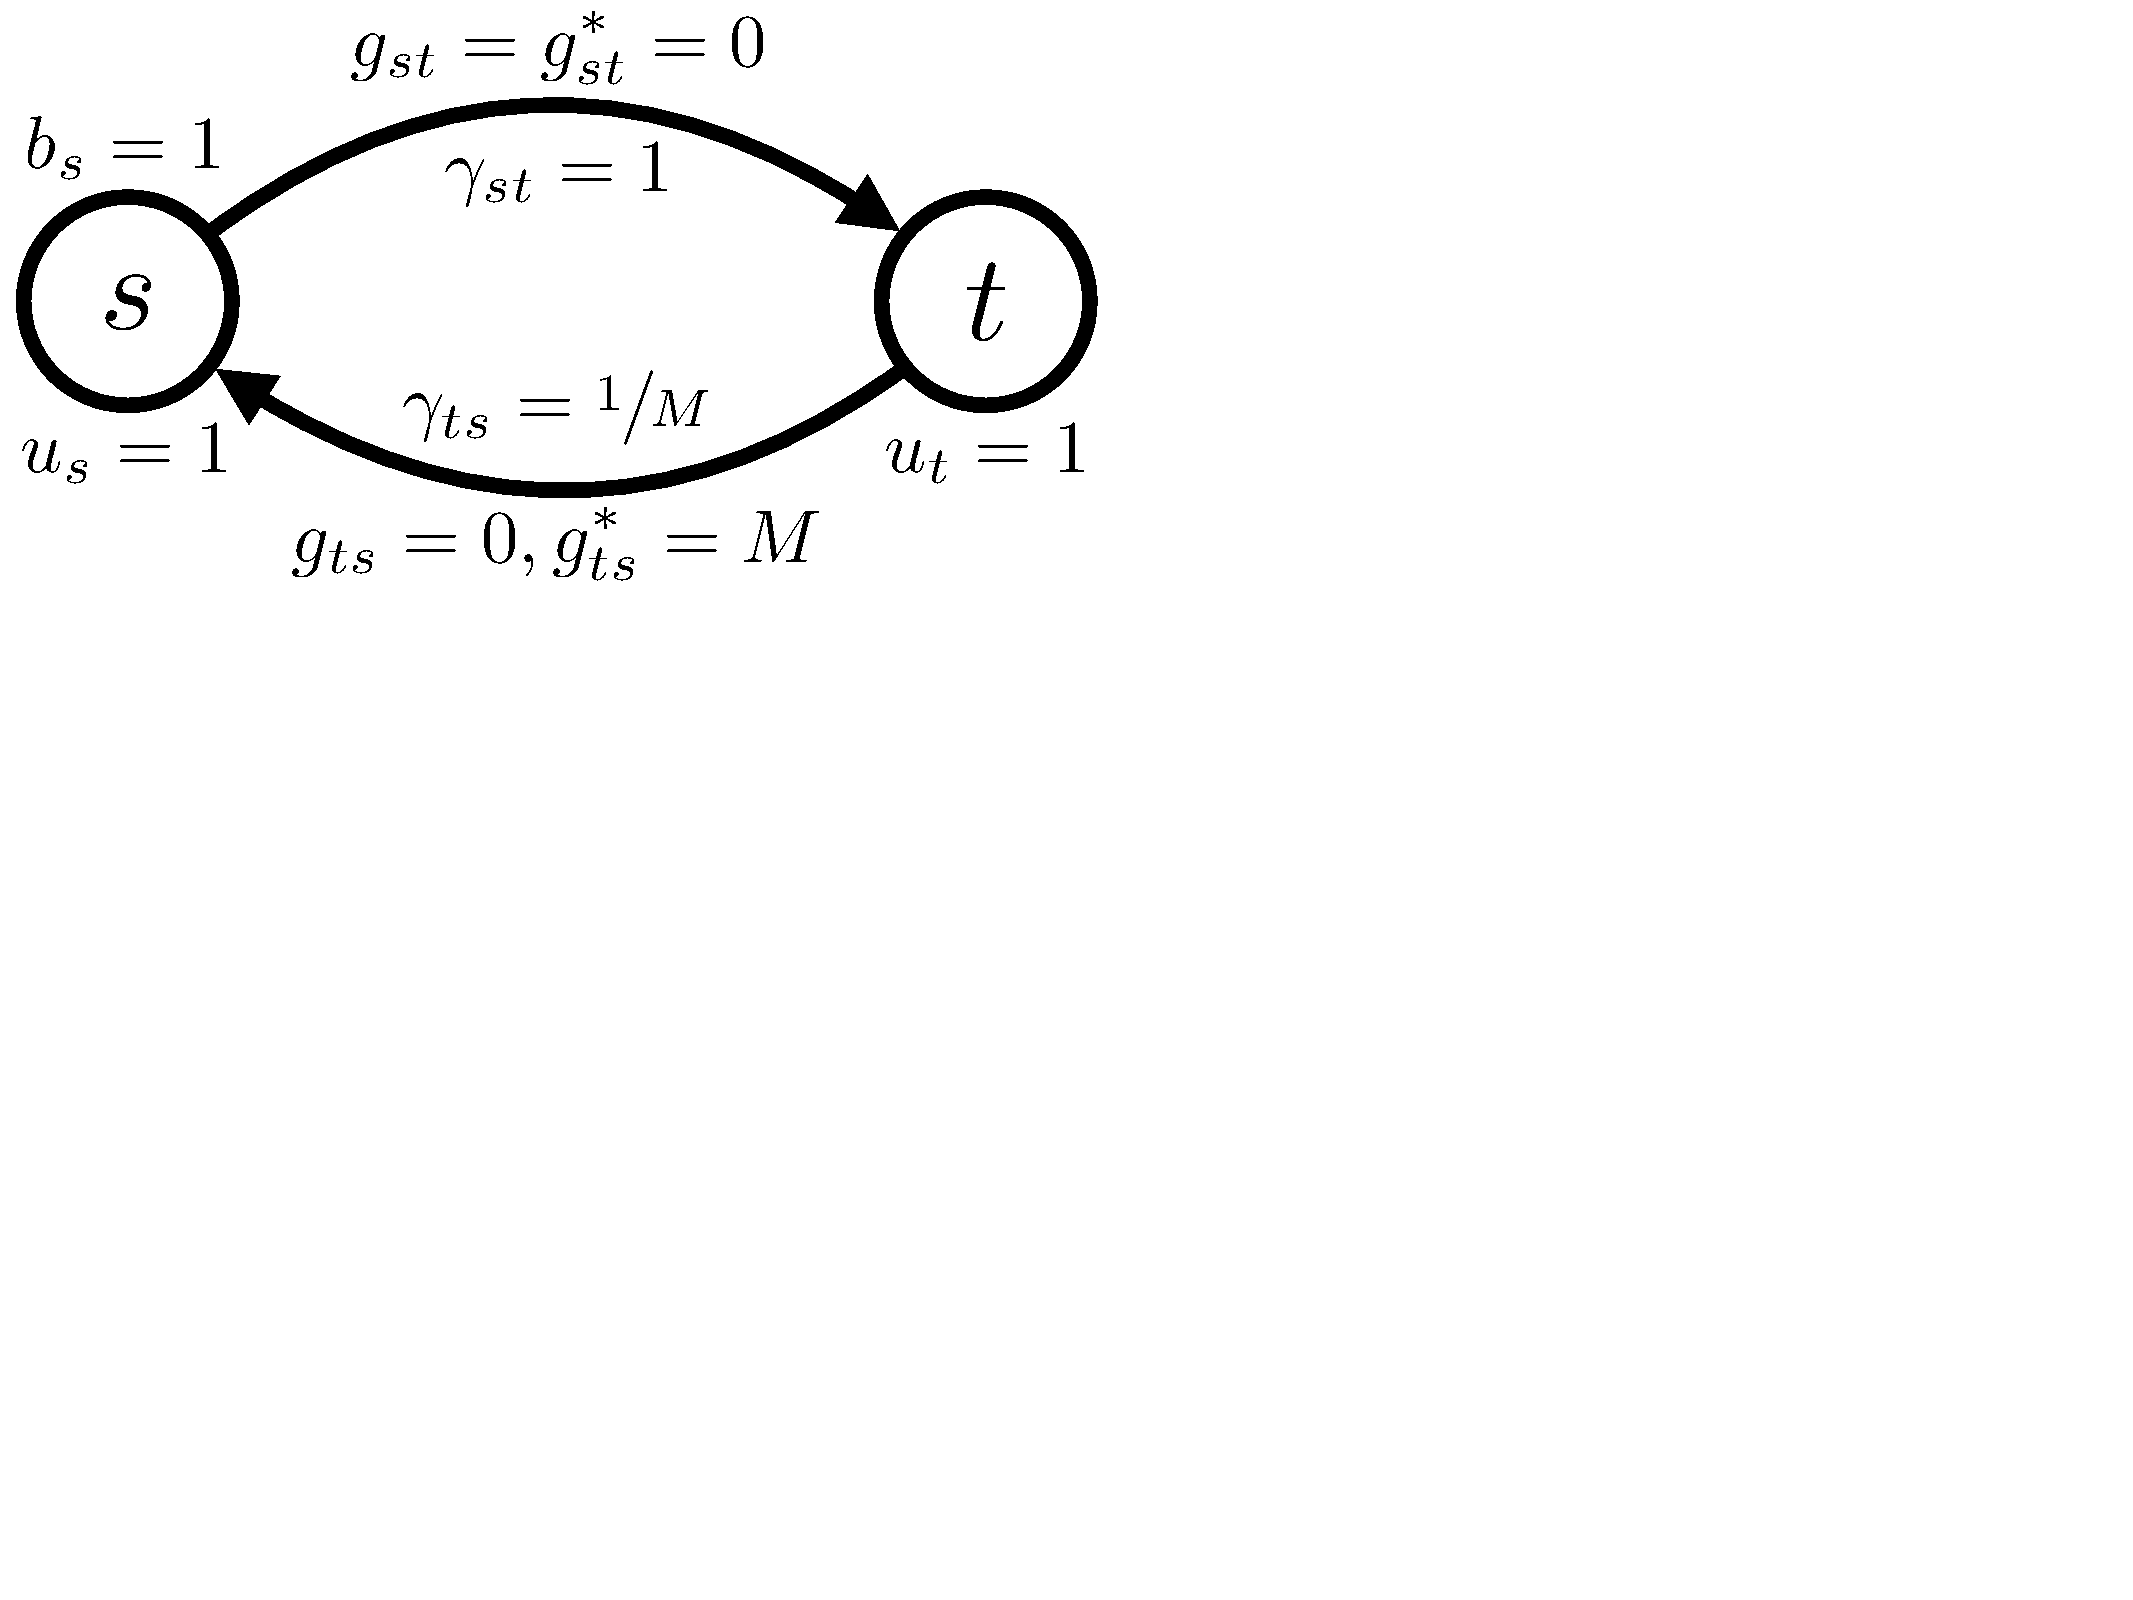
\includegraphics[width=0.45\textwidth]{figs/unsafe.pdf}
		\caption{
		\label{fig:unsafe}
		\rewrite{Simple example showing how unsafe $\mu$ causes problems.}\todo{Keep?}
		}
		\end{figure}

		\subsubsection{Subroutine: Producing Plentiful Nodes}
		\label{sec:sub-ppn}
		
		\begin{subroutine}
		For an input fitting pair $(f,u)$ without a plentiful node,
		continue executing the following two steps until at least one node becomes
		plentiful.
		\begin{enumerate}
		\item First, improve the primal solution by augmenting as much flow as possible,
		one unit at a time, along tight edges in the residual graph 
		from nodes with excess to either nodes with deficit, or the sink.
		It only augments along tight edges \rewrite{because}. Formally, let
		$D$ (``destinations'') be the union of the sink $t$ and all nodes with 
		deficit ($\nabla f_i^{\mu} < b_i^{\mu}$), and let $S$ (``sources'') be
		the set of all nodes that both have excess ($\nabla f_i^{\mu} \ge \lceil b_i^{\mu} \rceil$)
		and have a tight path in the residual graph to a node in $D$, then
		continue augmenting until $S$ is empty.
		\item Once it is not possible to augment any more flow, the second step scales down
		the labels and flow for all nodes and edges in $S$ by the same factor $\alpha$,
		which is chosen to be the largest value that \rewrite{does not violate} any of the dual
		constraints~(\ref{eq:dual}) or produces a plentiful node.
		\end{enumerate}
		\end{subroutine}

		\todo{RE-WRITE AS DJIKSTRAS}
		
		Although it is not necessary in practice, for clarify of explanation, one can think of choosing the scaling factor $\alpha$ as solving
		the following LP:
		\lpeq{\lpthree{max}
		{\alpha}
		{\gamma_{ij}^{\mu} \le 1\ \forall\ i,j \in \din(S)}
		{\nfiu - \biu \le 1}
		{\nexists\ \text{plentiful}\ i \in \vsink}
		}
		\begin{figure}[b!]
		\centering
		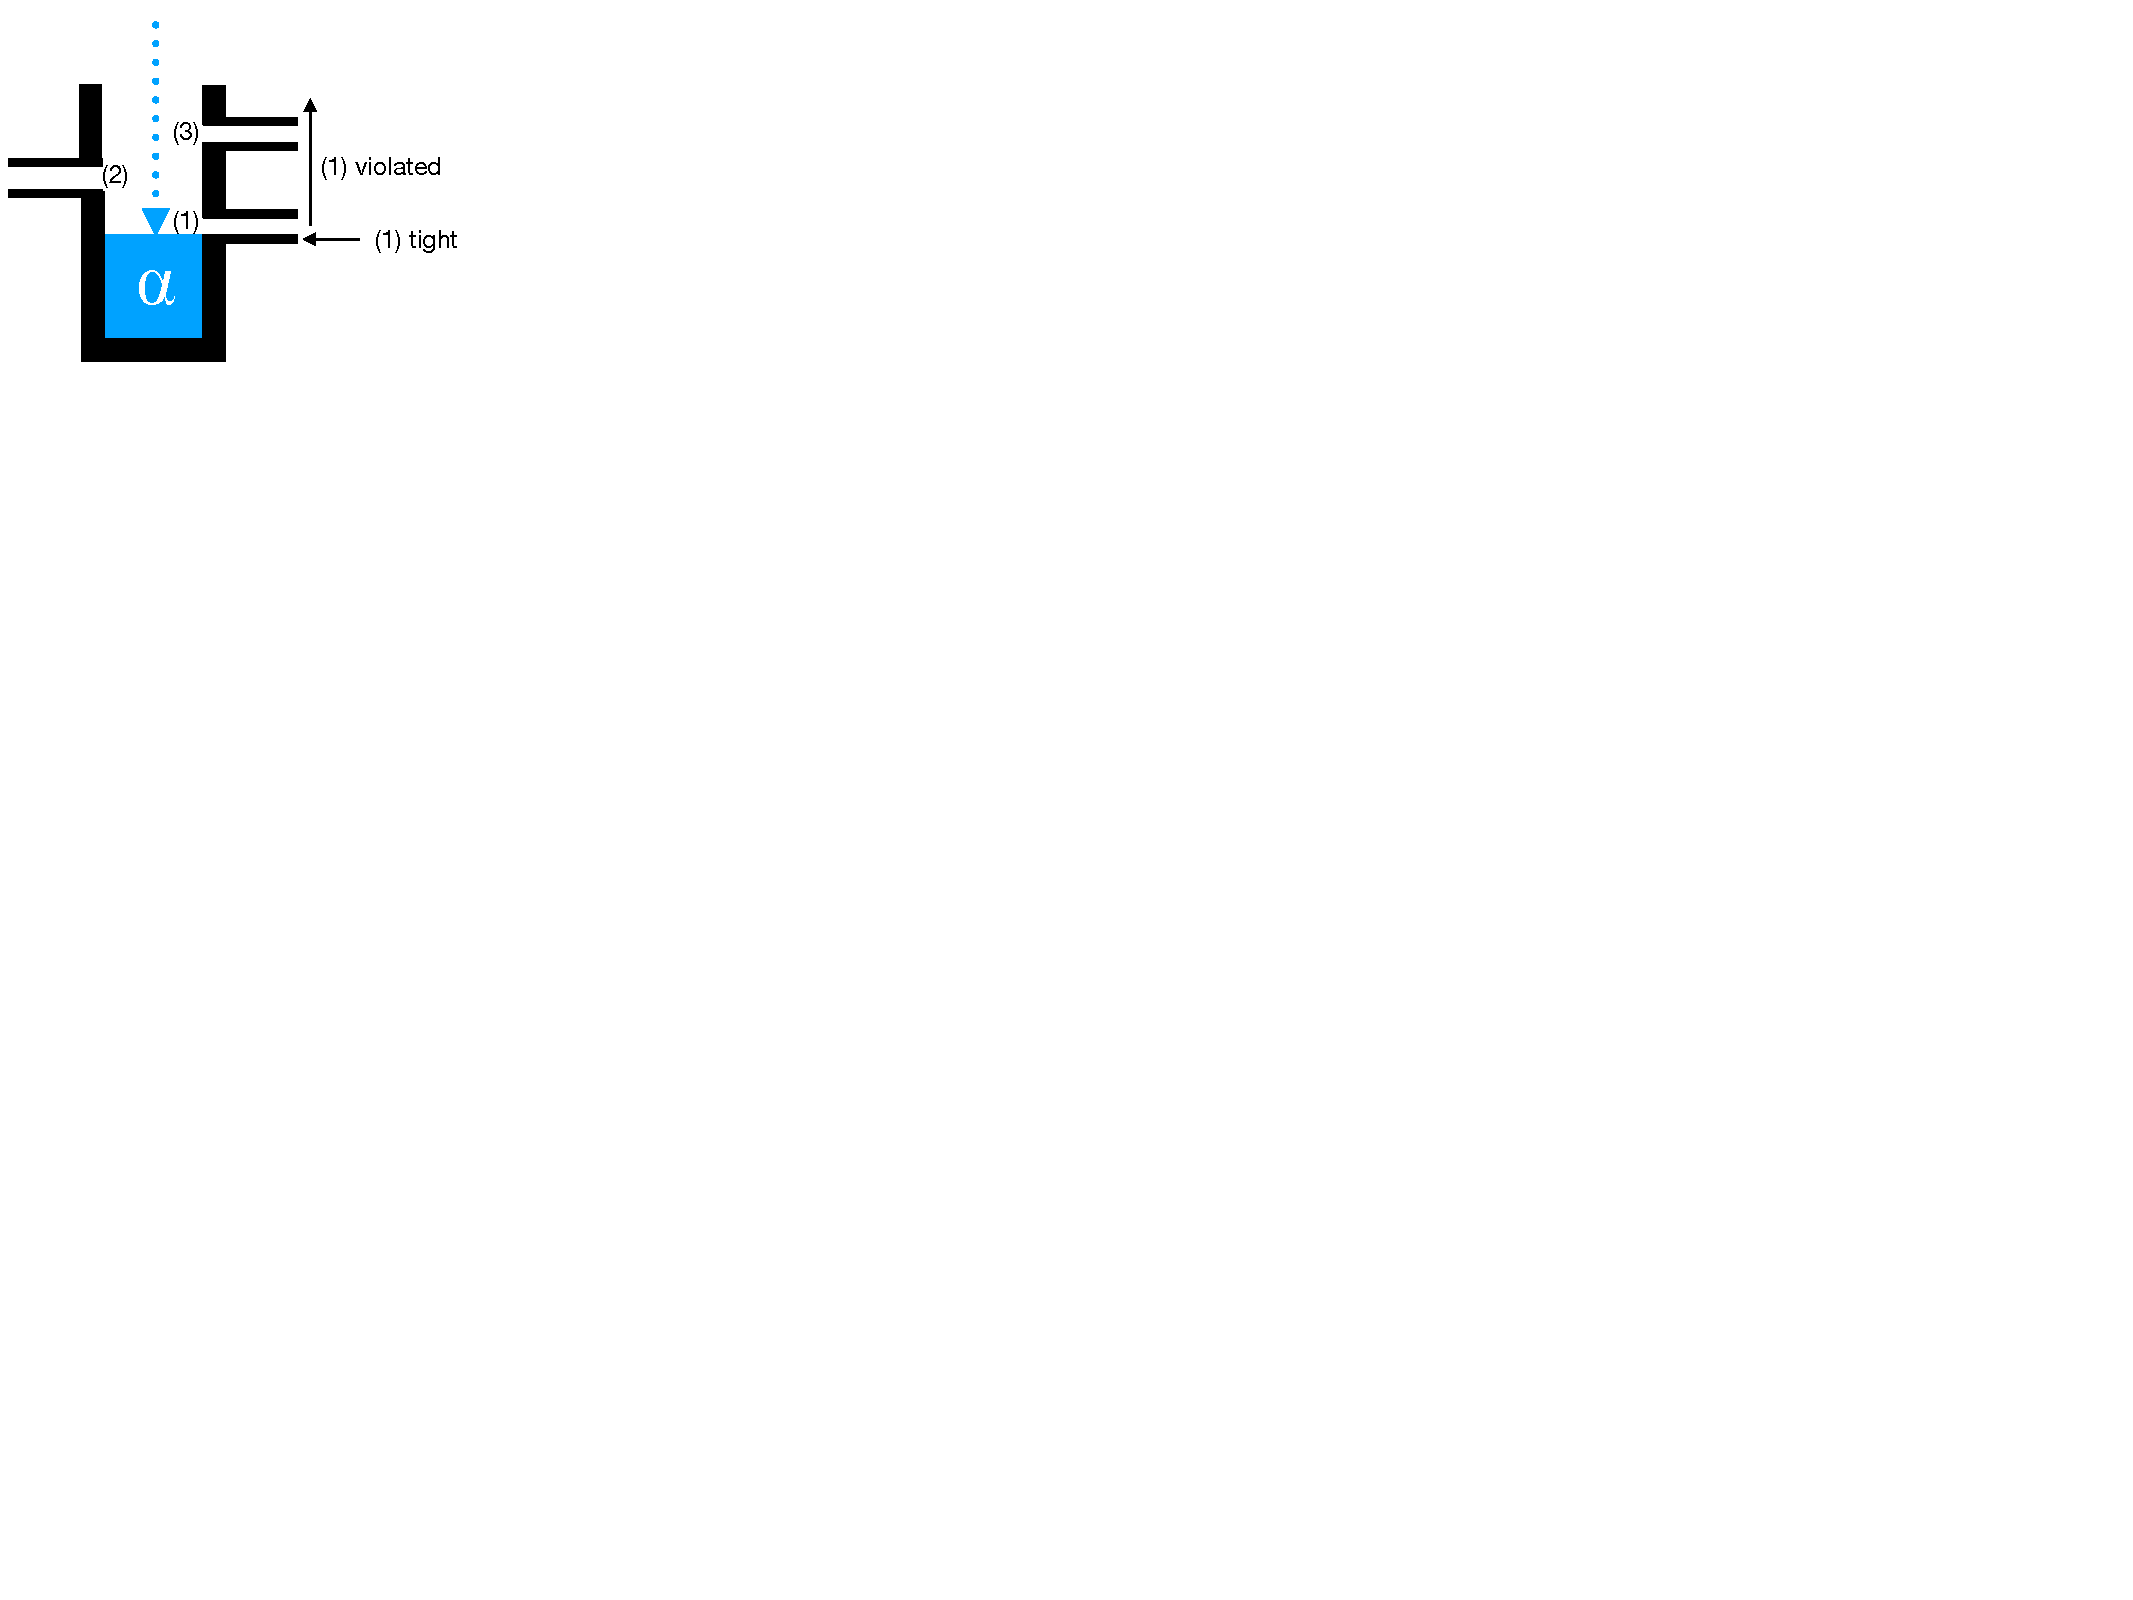
\includegraphics[width=0.35\textwidth]{figs/water.pdf}
		\caption{
		\label{fig:alpha}
		Informal analogy for the maximization of scaling parameter $\alpha$.
		Each pipe represents a constraint. $\alpha$ can only be increased until
		one of them becomes tight as increasing it further would leak into
		the lowest pipe and violate that constraint.
		At each step, the order of which constraint becomes tight first may be different.
		}
		\end{figure}
		Intuitively, as illustrated in Figure~\ref{fig:alpha}, this is akin to filling
		a basin with water as much as possible without any of the water leaking into one
		of three pipes, where each pipe represents a constraint and its height in the basin
		represents the value of $\alpha$ at which point it becomes tight.
		
		Thus, $\alpha$ is chosen such that one of the following constraints becomes
		tight, or, in other words, one of the following becomes true corresponding to
		each constraint, respectively:
		\begin{enumerate}[itemsep=-1mm]
			\item An edge entering $S$ becomes tight, and thus a new node is added to $S$
			\item A node in $S$ has excess $>1$, which allows us to augment flow from it
			\item A node becomes plentiful
		\end{enumerate}
		
		If (3) is true, we're done. If (1) or (2) are true, it ensures that we will now
		be able to make progress in the next iteration of the first step. Below, we show
		in Lemma~\ref{lem:scaling} that the augmentations in the first step similarly ensure
		that the algorithm can make progress in the second step. 
		
		Although it is conceptually easier to imagine increasing $\alpha$ continuously
		until one of these constraints becomes tight, in practice, it is possible to
		calculate $\alpha$ arithmetically in $O(n)$ by picking a value for each node
		that would satisfy one of the tightness conditions and then choosing the minimum
		such value so that only one of the constraints become tight and none are
		violated.
		The details of calculating the value are not particularly insightful so we omit them here, but the
		fact that it can be done is important for the running time analysis.
		
		We now make some important claims about the variables as the algorithm
		progresses that allow us to prove its correctness: i.e. that it terminates,
		producing a plentiful node.
		In the following section,
		we further prove that it terminates in strongly polynomial time and derive
		an upper bound on the running time.
		
		\begin{lemma}
		$f^{\mu}$ remains unchanged throughout the subroutine.
		\label{lem:fsame}
		\end{lemma} 
		\begin{proof}
			We must show that, for all edges $(i,j)$, $f_{ij}^{\mu}$ does not change.
			Recall that $f_{ij}^{\mu} = \frac{f_{ij}}{\mu_i}$. There
			are four possible cases for $(i, j)$:
			\begin{enumerate}
				\item Both outside of $S$. The subroutine only scales $i \in S$, so $\mu_i$ 
					does not change, and thus nor does $\fiju$.
				\item Both inside of $S$. The subroutine scales both $f_{ij}$ and $\mu$ by
					$\alpha$, which cancel each other out in the definition of $\fiju$.
				\item Only $i$ in $S$, which implies $i,j \in \dout(S)$. Then $f_{ij}=0$,
					because otherwise there would be a tight residual edge $j,i \in \din(S)$,
					and by definition $S$ has no incoming tight edges.
				\item Only $j$ in $S$, which implies $i,j \in \din(S)$. Again, incoming edges
					are not tight by definition of $S$ and we only augment along tight edges,
					so $f_{ij}$ is not augmented. Also, if $i \notin S$, then $\mu_i$ doesn't
					change. \qedhere
			\end{enumerate}
		\end{proof}
		\begin{corollary}
		$f^{\mu}$ is always integral.
		\end{corollary}
		\begin{proof}
		The augmentation step clearly maintains integrality of $f^{\mu}$ because we
		always augment by 1 unit at a time. The only other part of the algorithm that
		modifies the primal solution is the relabeling of $f_e$, and by
		Lemma~\ref{lem:fsame}, this never changes the value of $f^{\mu}$.
		\end{proof}
		\begin{lemma}
			\label{lem:scaling}
			For all nodes with non-zero demand in $S$, scaling $\mu$ in the second step
			strictly increases $|\biu|$. For all other nodes, $|\biu|$ remains unchanged.
			\todo{Show S cannot be empty?}
		\end{lemma}
		\begin{proof}
			First, trivially, scaling a node with zero demand cannot change its value
			($0\cdot\mu=0$), and the algorithm only updates $\mu_i$ for $i \in S$. Recall
			that $\biu$ is defined as $b_i / \mu_i$, and thus, if $\mu_i\leftarrow \mu_i / \alpha$,
			then
			\[ \biu \leftarrow \frac{b_i}{\mu_i / \alpha} = \alpha\frac{b_i}{\mu_i} = \alpha \biu. \] 
			Now it suffices to prove that $\alpha > 1$ always holds when any of the three
			constraints become tight.
			
			By construction, before rescaling, $S$ has no tight
			incoming edges. Recall $\giij = \gamma_i\frac{u_i}{u_j}$. In order for an
			incoming edge $i \notin S, j\in S$ to become tight (1), we must have $\giij=1$:
			since we only scale values in $S$, $\alpha$ must be ${1}/{\giij}$, which is
			always greater than $1$ because $\giij < 1$ (by the feasibility of the dual).
		
			From the terminating condition of the augmentation step (the lack of any nodes
			in $S$ having excess), we know $\Ex(f) = \nfiu - \biu < 1$. Since, by
			Lemma~\ref{lem:fsame}, $\nfiu$ is unchanged and only nodes in $\vsrc$ (i.e. $b_i<0$)
			can have excess, the only way for to make $\Ex(f) \ge 1$ is if $\biu$ becomes
			more negative, which only happens if $\alpha > 1$. 
			
			Finally, we start out with the assumption that there are no plentiful nodes.
			In order for a node to become plentiful (3), its demand $\biu$ must increase,
			which is only possible if $\alpha > 1$.
		\end{proof}
		\begin{lemma}
			\label{lem:still-fit}
			$\fp$ remains a fitting pair throughout the subroutine.
		\end{lemma}
		\begin{proof}
			In order to be a fitting pair, we must have the following relationship between
			$f$ and $\mu$: for all $(i, j) \in E$, $\giij \leq 1$, and when $f_{ij} > 0$, 
			$\giij = 1$. \todo{This is a definition, not a proof.}
		\end{proof}
		
		\begin{lemma}
			The rescaling of $\mu$ during produce-plentiful-node does not break 
			the safety of $\mu$, i.e. there is a corresponding feasible primal
			solution even though we haven't kept track of it.
			\todo{Why is this here:} (~\ref{lem:usafe})
		\end{lemma}
		\begin{proof}
		The initialization subroutine is guaranteed to produce a fitting pair $\fp$,
		where $f$ is feasible, so we have that initially $\mu$ is safe. Now assume $\mu$
		is safe before running the subroutine. For sake of contradiction, assume that
		after running the subroutine, the updated labeling $\mu'$,
		is no longer safe. That is, there exists some subset of vertices $X \subseteq \vnott$  
		without any incoming tight edges ($\{\gamma_e^{\mu'} = 1\ \forall\ e \in \din(X)\} = \varnothing$)
		and where all nodes have positive demand $b^{\mu'}(X) > 0$.
		
		Suppose we divide $X$ into two parts: the subset of vertices in $S$, $X \cap S$, and those
		not in $S$, $X \setminus S$. Recall that $\mu_i' = \frac{\mu}{\alpha}$ for $i\in S$
		and $\mu' = \mu$ for $i \notin S$. Then we can rewrite the node demands under $\mu'$
		in terms of the demands under $\mu$ as follows:
		$$b^{\mu'}(X) = \frac{1}{\alpha}b^{\mu}(X \cap S) + b^{\mu}(X \setminus S)$$
		If, as we assumed, $b^{\mu'}(X) > 0$, then either $b^{\mu}(X \cap S)$ or 
		$b^{\mu}(X \setminus S)$ must be positive.
		\todo{Fill in details. $\mu'$ is defined in terms of $S$.}
		Now consider the set of edges coming into each of these subsets...
		Any edge that's tight under $\mu'$ was tight under $\mu$, because $\geu$, if
		it has no tight edges under $\mu'$ then it also had no tight edges under
		$\mu$.
		
		Therefore, since neither of the two parts of $X$
		have any tight incoming edges under $\mu$ and at least one of them
		must have strictly positive node demands, at least one of them
		violates the safety conditions of $\mu$ and thus $\mu$ was not safe.
		This is a contradiction, and thus if $\mu$ was safe, $\mu'$ must also be safe.
		
		\end{proof}
		
		In summary, we have shown that the primal and dual steps always allow room for the other to make progress, and collectively each iteration of the two steps strictly increases $|\biu|$ towards
		the definition of a plentiful node. Thus, the subroutine will eventually produce one. We have also shown that the updates it makes to $f$ and $\mu$ do not violate any of the previous conditions stated for being able to ultimately derive a primal optimal solution once our fitting pair finds the dual optimal. 
		
		\subsubsection{Running Time Analysis}
		The algorithm consists of three basic types of operations: scaling, augmentation, and contraction.
		The number of contractions is bounded by $n$. Contraction itself
		requires computing a regular flow and performing a bounded number of graph operations, but
		strongly polynomial algorithms already exist for these. So the goal is to bound the running time
		(number of arithmetic operations) between any two contractions.
		
		Augmentation itself consists of a graph search on the tight subgraph, an $O(m)$ operation.
		Between rounds of augmentation, there is a scaling round. Each atomic scaling step stops
		when either (i) a node has become plentiful, leading to a contraction; (ii) a node has an
		excess greater than $1$, leading to a new augmentation round; or (iii) the loose cut
		$S$ has been extended by at least one node. (iii) can only happen at most $n$ times; thus,
		there are at most $n$ scaling steps between any two augmentations. Each scaling step
		is an $O(n)$ operation, leading to a na\"ive time bound of $O(n^2)$ between any two augmentations.
		This can be improved to $O(m + n \log n)$ by applying the framework of Dijkstra's
		algorithm with costs $-\log \gamma^u_e$. The loose cut $S$ corresponds to the expanding
		frontier of Dijkstra's algorithm.
		
		It remains to bound the total number of augmentations the algorithm may perform. We'd
		like to show that after a strongly polynomial number of augmentations, the algorithm
		is guaranteed to find a plentiful node.
		
		\begin{lemma} \label{lem.num-aug}
			After $O(mn)$ augmentations, the algorithm is guaranteed to find a plentiful node.
		\end{lemma}
		First, a preliminary lemma. We denote the period between successive contraction
		steps as an epoch.
		\begin{lemma}
		At any node $i \in \vsrc$, the deficit is at most one. Moreover, at most one augmentation
		ends at such a node during any epoch.
		\end{lemma}
		\begin{proof}
			At the beginning of the algorithm, the flow is feasible, so $\nfiu - \biu \geq 0$.
			Rounding decreases $\nfiu$ by less than one. Similarly, during each contraction,
			the adjusted flow is computed with $nabla g_i^\mu \geq \lfloor \biu \rfloor$ everywhere.
			
			Between contractions, the deficit can be modified by scaling and augmentation steps.
			Since $i \in \vsrc$, $\biu < 0$, and so $\biu$ can only decrease during scaling.
			Meanwhile, augmentations only decrease deficits.
			Once $\nfiu \geq \biu$, no augmentation ending at $i$ will be contemplated unless $i$
			experiences a deficit again. The only way for this to happen would be for
			augmentations beginning at $i$ to reduce $\nfiu$ below $\biu$. However,
			an augmentation will only begin at $i$ if
			$\nfiu - \biu \geq 1$, and will reduce $\nfiu$ by exactly one. Hence, $i$ will
			never again experience a deficit during the epoch, and so there will be no further
			augmentations ending at $i$.
		\end{proof}
		
		\begin{proof}[Proof of Lemma \ref{lem.num-aug}]
		Define two potential functions
		\begin{align*}
		\Psi(\mu) &= - \sum_{i \in \vsrc} \biu \\
		\Phi(\mu) &= \sum_{i \in \vsrc} \nfiu + \Psi(\mu) = \sum_{i \in \vsrc} \nfiu - \biu
		           \leq \Ex(\mu)
		\end{align*}
		\todo{complete proof}
		\end{proof}


	\subsection{Contraction}

	Once we have produced a plentiful node, finding a contractible edge is straightforward. 

	The purpose of contraction is that it reduces the size of the graph by one node,
	which puts a strongly polynomial bound of $n$ on the number of contraction
	operations.
	\subsection{Expand to Original}
	\subsection{Compute Primal}
	\subsection{Amortized Analysis}


\section{Discussion and Future Work}

	\subsection{Non-triviality of a strongly polynomial algorithm}

	\todo{Explain} why applying ideas from strongly polynomial algorithms for
	min-cost flow was not straightforward. 



\setlength{\bibitemsep}{0pt}
\nocite{*}
\printbibliography
\end{document}
 
